\documentclass[12pt]{article}
\usepackage[dot, autosize, outputdir="dotgraphs/"]{dot2texi}
\usepackage{tikz}
\usetikzlibrary{shapes}
\usepackage[utf8]{inputenc}
\usepackage{amsmath}
\usepackage{mathtools}
\usepackage{amsfonts}
\usepackage{lastpage}
\usepackage{pdfpages}
\usepackage{gauss}
\usepackage{fancyvrb}
\usepackage{fancyhdr}
\usepackage{graphicx}
\pagestyle{fancy}
\fancyfoot[C]{\footnotesize Page \thepage\ of 8}
\DeclareGraphicsExtensions{.pdf,.png,.jpg}
\title{Oversætter}
\author{Nikolaj Dybdahl Rathcke}
\chead{Nikolaj Dybdahl Rathcke (rfq695)}

\begin{document}
\section*{Oversætter - Week 1}

\subsection*{1 - DFA Minimisation}
We are given a DFA that we wish to minimize.\\
We split it into 2 sets, $G1$ with states $F$ and $G2$ with states $S\setminus F$.
\begin{align*}
G_1 &= \{3\}\\
G_2 &= \{1,2,4,5,6,7,8\}
\end{align*}
We check if the groups are consistent. We see that $G1$ is consistent since it consists of only 1 element. However $G2$ might not be.
\begin{center}
\begin{tabular}{|c|c|c|}
\hline 
G2 & 0 & 1 \\ 
\hline 
1 & G2 & G2 \\ 
\hline 
2 & G2 & G1 \\ 
\hline 
4 & G1 & G2 \\ 
\hline 
5 & G2 & G2 \\ 
\hline 
6 & G1 & G2 \\ 
\hline 
7 & G2 & G2 \\ 
\hline 
8 & G2 & G1 \\ 
\hline 
\end{tabular}
\end{center}
We see that it's not consistent so we split it into maximal consistent subgroups, so that
\begin{align*}
G_1 &= \{3\}\\
G_3 &= \{1,5,7\}\\
G_4 &= \{2,8\}\\
G_5 &= \{4,6\}
\end{align*}
The procedure\footnote{Algorithm 1.4} is repeated for $G3$ we get
\begin{center}
\begin{tabular}{|c|c|c|}
\hline 
G3 & 0 & 1 \\ 
\hline 
1 & G4 & G5 \\ 
\hline 
5 & G4 & G5 \\ 
\hline 
7 & G3 & G3 \\ 
\hline 
\end{tabular}
\end{center}
So we get
\begin{align*}
G_1 &= \{3\}\\
G_4 &= \{2,8\}\\
G_5 &= \{4,6\}\\
G_6 &= \{1,5\}\\
G_7 &= \{7\}
\end{align*}
and using Algorithm 1.4 on $G4, G5$ and $G6$ we get
\begin{center}
\begin{tabular}{|c|c|c|}
\hline 
G4 & 0 & 1 \\ 
\hline 
2 & G7 & G1 \\ 
\hline 
8 & G7 & G1 \\ 
\hline 
\end{tabular}
\end{center}
\begin{center}
\begin{tabular}{|c|c|c|}
\hline 
G5 & 0 & 1 \\ 
\hline 
4 & G1 & G7 \\ 
\hline 
6 & G1 & G7 \\ 
\hline 
\end{tabular}
\end{center}
\begin{center}
\begin{tabular}{|c|c|c|}
\hline 
G6 & 0 & 1 \\ 
\hline 
1 & G4 & G5 \\ 
\hline 
5 & G4 & G5 \\ 
\hline 
\end{tabular}
\end{center}
The last 2 are singletons and therefore all are consistent.\\
The minimized DFA is shown below drawn with the program Graphviz.\\
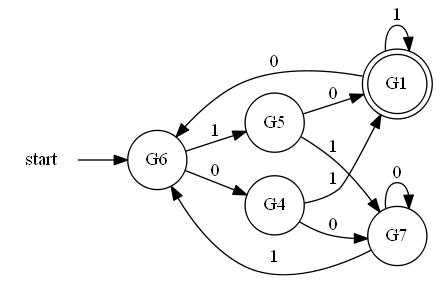
\includegraphics[scale=0.6]{graph1}

\newpage

\subsection*{2 - Backtracking Automaton}
We are given three regular expressions
\begin{align*}
a_1 &= ab^*\\
a_2 &= a^*b\\
a_3 &= (ab)^*c
\end{align*}

\subsubsection*{a}
Give an NFA for each expression and construct a combined NFA.\\
\\
For $ab^*$\\
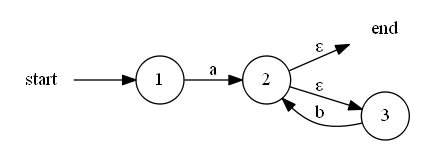
\includegraphics[scale=1]{graph2}\\
for $a^*b$\\
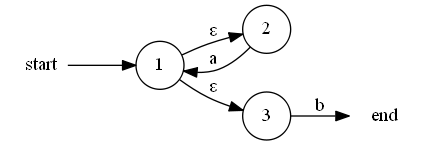
\includegraphics[scale=1]{graph3}\\
for $(ab)^*c$\\
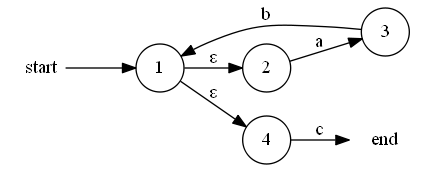
\includegraphics[scale=1]
{graph4}\\
\newpage
Below is the combined NFA with superfluous epsilon transitions removed.\\
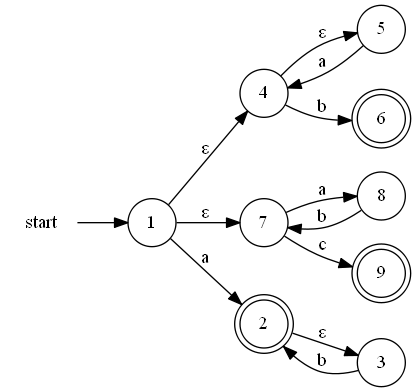
\includegraphics[scale=0.6]{graph5}

\subsubsection*{b}
We wish to convert this NFA to DFA by subset construction.\\
We begin by adding all epsilon transitions we can reach from state 1 to $s'_0$ and then call \textit{move}\footnote{Algorithm 1.3} on this set.
\begin{align*}
 s'_0 &=\{1,4,5,7\}\\
 \\
 s'_1&=move(s'_0,a) \\
 &=\{2,3,4,5,8\} \\
 \\
 s'_2&=move(s'_0,b) \\
 &=\{6\} \\
 \\
 s'_3&=move(s'_0,c) \\
 &=\{9\}
\end{align*}
Proceeding with the function \textit{move} on $s'_1$
\begin{align*}
 s'_4&=move(s'_1,a) \\
 &=\{4,5\} \\
 \\
 s'_5&=move(s'_1,b) \\
 &=\{2,3,6,7\} \\
 \\
 s'_6&=move(s'_1,c) \\
 &=\{\}
\end{align*}
And for $s'_2$ and $s'_3$ it is easy to see that all sets coming from them are empty sets.\\
We use \textit{move} on $s'_4$
\begin{align*}
 s'_6&=move(s'_4,a) \\
 &=\{4,5\} \\
 \\
 s'_7&=move(s'_4,b) \\
 &=\{6\} \\
 \\
 s'_8&=move(s'_4,c) \\
 &=\{\}
\end{align*}
Since $s'_7$ is the same this set is not included but $s'_4$ points to itself and that $s'_8$ is the same as $s'_2$, so we have no new sets and $S'=\{s'_0,s'_1,s'_2,s'_3,s'_4\}$.\\
For $s'_5$ we get
\begin{align*}
 s'_{6}&=move(s'_5,a) \\
 &=\{8\} \\
 \\
 s'_{7}&=move(s'_5,b) \\
 &=\{2,3\} \\
 \\
 s'_{8}&=move(s'_5,c) \\
 &=\{9\}
\end{align*}
The new sets are $s'_{6}$ and $s'_{7}$ and $s'_8$ is the same as $s'_3$. We can tell that $s'_{7}$ will point to itself if $move(s'_{7},b)$ is called and the other sets are empty. $s'_{6}$ will make a new set if $move(s'_{6},b)$ is called so
$$s'_{8}=\{7\}$$
Which can point back to $s'_6$\\
So $S'=\{s'_1,s'_2,s'_3,s'_4,s'_5,s'_{6},s'_{7},s'_{8}\}$ and the constructed DFA is seen below\\
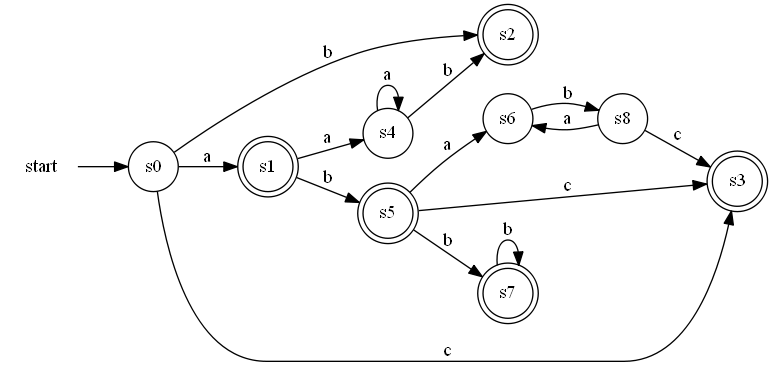
\includegraphics[scale=0.5]{graph6}
\subsubsection*{c}
Describe the transitions and backtracking used when the combined DFA analyzes the input 'ababacca'.\\
\\
It starts in $s'_0$\\
Goes to $s'_1$ (a), goes to $s'_5$ (b), goes to $s'_6$ (a), goes to $s'_8$ (b), goes to $s'_6$ (a)\\
And it cannot take a 'c' route and $s'_6$ is not an accepting state, so it backtracks to the last accepting state which is 'ab'\\
\\
The input is then 'abacca'.\\
It goes to $s'_1$ (a), goes to $s'_5$ (b), goes to $s'_6$ (a).\\
And fails at 'c', and backtracks to the last accepting state which is 'ab'.\\
\\
The input is then 'acca'.\\
It goes to $s'_1$ (a).\\
And there is no 'c' route but it is in an accepting state.\\
\\
The input is then 'cca'.\\
It goes to $s'_3$ (a).\\
And there is no 'c' route but it is in an accepting state.\\
\\
The input is then 'ca'.\\
It goes to $s'_3$ (a).\\
And there is no 'a' route but it is in an accepting state.\\
\\
The input is then 'a'.\\
It goes to $s'_1$ (a).\\
Which is the end and it is in an accepting state.\\
\\
So it analyzes it to be 'ab', 'ab', 'a', 'c', 'c', 'a'. 

\newpage

\subsection*{Mosmllex Scanner Construction}
The output for the scanner is: 'ab', 'ab', 'a', 'c', 'c', 'a'.\\
This is the same that was got in (2c).

\subsection*{More on Regular Languages and Tokenisation}
\subsubsection*{a}
Using the alphabet of decimal digits, give regular expressions describing the following languages\\
\\
\textit{i: Numbers divisible by 5.}\\
$$[0-9]^*[05]$$
\textit{ii: Numbers in which digit 5 occurs exactly three times.}
$$[0-46-9]^*5[0-46-9]^*5[0-46-9]^*5[0-46-9]^*$$
\subsubsection*{b}
Are the following languages over the alphabet of decimal digits regular? Give short convincing reasons for your answers.\\
\\
\textit{i: Numbers which contain digit '1' exactly as many times as digit '2'.}\\
\\
This language is not regular since it can contain infinite 1's and infinite 2's and you cannot match on a number that potentially can be infinitely long.\\
\\
\textit{ii: Numbers N$<$1000000 which contain digit '1' exactly as often as digit '2'.}\\
\\
This language is regular since it has a finite amount of numbers (assuming these are natural numbers) so it is possible to match on a number.

\end{document}
